\documentclass[paper=a4,fontsize=12pt]{scrartcl}
\usepackage{geometry}
\usepackage{graphicx}
\usepackage{wrapfig}
\usepackage{titling}
\usepackage{float}
\usepackage{xargs}
\usepackage[format=plain]{caption}
\geometry{verbose, a4paper, tmargin=25mm, bmargin=25mm, lmargin=25mm, rmargin=25mm}

\usepackage[utf8]{inputenc}
\usepackage[ngerman]{babel}
\usepackage{fancyhdr} %Paket laden
\pagestyle{fancy} %eigener Seitenstil
\fancyhf{} %alle Kopf- und Fußzeilenfelder bereinigen
\fancyhead[L]{
\includegraphics[width=3cm]{img/logo_bfh_de.jpg}} %Kopfzeile links
\fancyhead[C]{} %zentrierte Kopfzeile
\fancyhead[R]{Janosch Rohdewald, Marco Füllemann} %Kopfzeile rechts
\renewcommand{\headrulewidth}{0.4pt} %obere Trennlinie
\fancyfoot[C]{\thepage} %Seitennummer
\renewcommand{\footrulewidth}{0.4pt} %untere Trennlinie

\title{Wo ist Walter}
\author{Marco Füllemann\newline Janosch Rohdewald}
\date{3. Dezember 2014}

% Text mit Bild links
\newcommandx{\descFig}[5][1=0.5, 2=0.45]{
  \noindent
  \begin{minipage}[t][][b]{#1\textwidth}
    #5
  \end{minipage}
  \hspace{0.05\textwidth}
  \begin{minipage}[t][][t]{#2\textwidth}
    \begin{figure}[H]
      \vspace{-1em}
      \includegraphics[width=1\textwidth]{#3}
      \caption{#4}
    \end{figure}
  \end{minipage}
  \newline\newline
}



\begin{document}
% Title page
\pagestyle{empty}
\hbox{ % Horizontal box
  \hspace*{0.2\textwidth} % Whitespace to the left of the title page
  \rule{1pt}{\textheight} % Vertical line
  \hspace*{0.05\textwidth} % Whitespace between the vertical line and title page text
  \parbox[b]{0.75\textwidth}{ % Paragraph box which restricts text to less than the width of the page

  {\noindent\Huge\bfseries \thetitle}\\[2\baselineskip] % Title
  {\large \textit{Suche mit Hilfe von Bild-Operatoren in Matlab}}\\[4\baselineskip] % Tagline or further description
  {\Large \textsc{\theauthor}} % Author name
  \vspace{0.5\textheight} % Whitespace between the title block and the publisher
  }}
\newpage

% Content
\pagestyle{fancy}
\section*{Zusammenfassung}
In dieser Arbeit wurde mittels Computer-Perception-Algorithmen versucht Walter in einem "Wo ist Walter"\--Bild zu finden. Zu diesem Zweck wurden Pullover und Brille extrahiert um mögliche Positionen zu finden.
\section*{Einleitung}
Um Walter zu erkennen wurden in zwei unabhängigen Schritten sein Pullover und seine Brille extrahiert. Bei der Brillenextraktion wurde eine Kreis-Hough-Transformation mit bestimmten Radien angewandt. Bei der Extraktion seines Pullovers wurden die Farben des Pullovers extrahiert, nach erfolgter Dilatation wurde ein spezifisches Region-Growing durchgeführt.
\section*{Grundlagen}
\subsection*{Farbkanal Extraktion}
Eine Farbkanal Extraktion ist eine simple Operation, welche die einzelnen Farbkanäle (Rot, Grün, Blau), eines Bildes extrahiert und separat zur Verfügung stellt. Mit diesen Daten können beispielsweise die roten Pixel in einem Bild gefunden werden.
\subsection*{Morphologische Operatoren}
Morphologische Operatoren sind ein Teil von lokalen Operatoren. Lokale Operatoren beziehen für die Berechnung eines neuen Wertes eines Pixels nicht nur das zugrundeliegende Pixel bei, sondern auch seine Region.\\
In der Bildverarbeitung können morphologische Operationen auf Binär- und Graustufenbilder angewendet werden und sind für vielfältige Bildverarbeitungsaufgaben wie Kantenextraktion, Skelettierung oder Segmentierung geeignet. Beispiele eines morphologischen Operators sind die Dilatation oder Erosion, wobei Lücken von Pixelwerten geschlossen resp. geöffnet werden. 
\subsection*{Hough Transformation}
Die Hough-Transformation (HT) ist eine globale Transformation, die gebraucht wird, um
geometrische Strukturen wie Geraden, Kreise und Ellipsen in einem bereits binarisierten
Bild zu detektieren. Der Algorithmus geht auf Paul Hough zurück, der das Verfahren 1962
patentieren liess.
Wie bei allen globalen Transformationen üblich, ist auch die Hough-Transformation in
ihrer einfachen Variante eine rechenintensive Aufgabe. Positiv ist, dass sie sehr robust
und wenig anfällig gegen Rauschen ist.
\subsection*{Region-Growing}
Beim Region-Growing wird ein bestimmtes Pixel gewählt, von diesem aus werden seine Nachbarn analysiert. Wenn die Nachbarn ein bestimmtes Kriterium erfüllen (z.B. Schwellwert) werden sie zur Region hinzugefügt. Für die hinzugefügten Pixel werden wieder die Nachbarn gewählt und analysiert usw.
\newpage
\section*{Vorgehen, Methoden, Analysen}
Wir haben unser Vorgehen auf den bereits erlernten Grundlagen in der CPVR-Vertiefung des Studiums aufgebaut. Dabei wollten wir die Aufgabe nicht mit Hilfe einer Ähnlichkeitssuche von Walters Bild lösen. Wir haben uns entschieden wichtige Merkmale von Walter durch die Anwendung von lokalen und globalen Operatoren zu finden. Dabei ist wichtig zu erwähnen, dass es dadurch nicht möglich ist Walter anhand eines einzigen Merkmals zu finden. Deshalb wurde der Ansatz gewählt die Brille durch eine Kreis-Hough Transformation zu finden und das T-Shirt durch das horizontale rot-weiss Muster.
\subsection*{Brille}
Um eine einfachere Entwicklung des Algorithmus zu ermöglichen, wurde mit einem Ausschnitt des Bildes gearbeitet, welcher wie folgt gewählt wurde:

\begin{figure}[htbp]
\centering
\begin{minipage}{.5\textwidth}
  \centering
  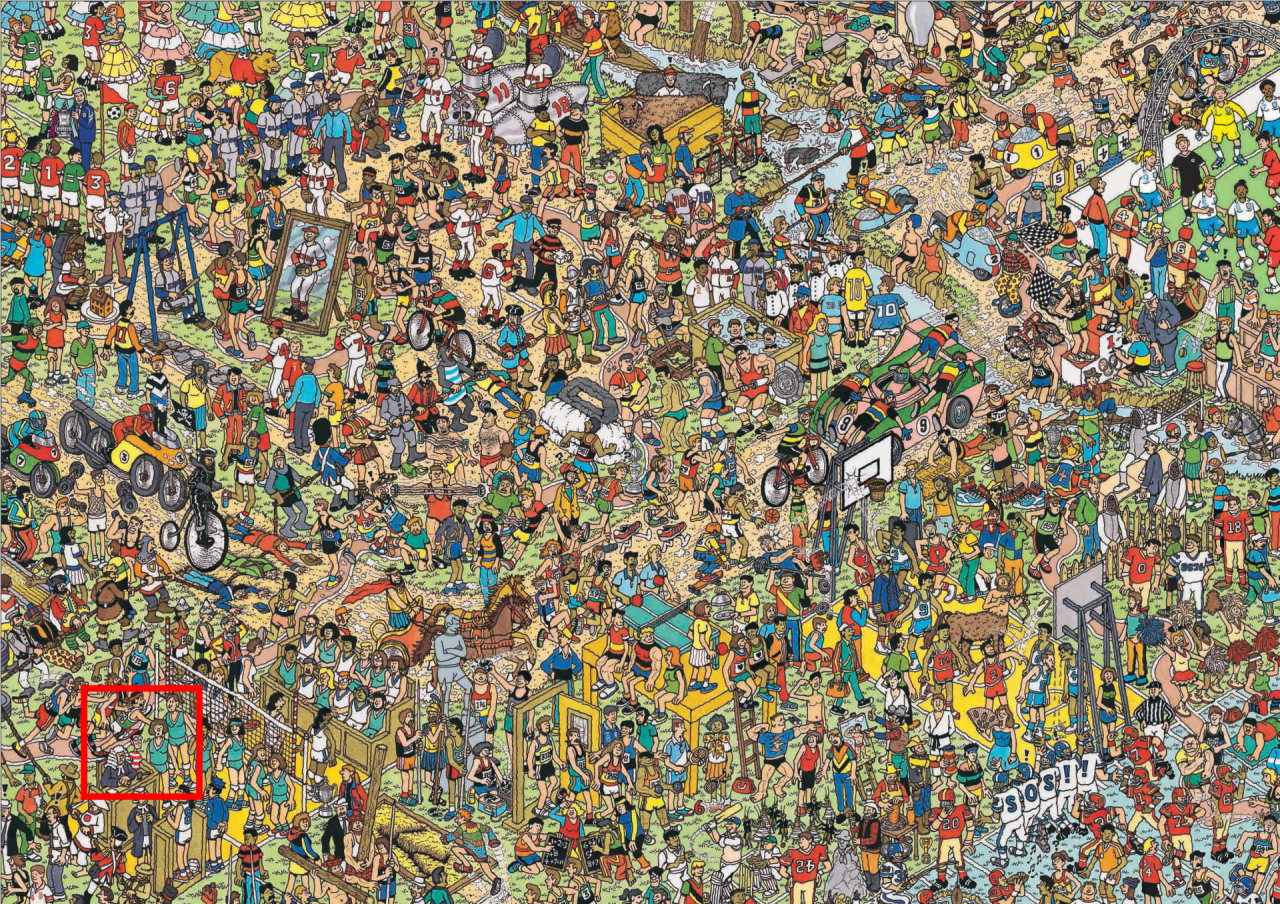
\includegraphics[height=.6\linewidth]{img/WallyWembleyGlassesSelection.png}
  \caption{Wembley Stadion}
\end{minipage}%
\begin{minipage}{.5\textwidth}
  \centering
  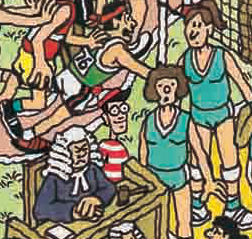
\includegraphics[height=.6\linewidth]{img/WallyWembleyCroppedGlasses.png}
  \caption{Ausschnitt Brillendetektion}
\end{minipage}
\end{figure}
\subsubsection*{Brillenglasränder} 
Die erste Idee war die Brille durch eine Extraktion der Brillenglasränder zu finden.

\descFig{img/glasses_1_blackExtract.jpg}{Extraktion der schwarzen Farbe}{Dafür wurden zuerst die (schwarzen) Pixel, bei welchen alle 3 RGB Kanäle Werte kleiner als 0.3 (Hex 0x4C) besitzen, extrahiert.}
\descFig{img/glasses_1_closing.jpg}{Closing Operation}{Die Ränder der Brillengläser sind leider nicht nur schwarz, sondern gehen auch in einen Braunton über. Um die Lücken im Brillenrand zu schliessen wurde ein Closing Operator angewandt; dies bedeutet eine Dilatation gefolgt von einer Erosion.}
\descFig{img/glasses_1_canny.jpg}{Canny edge detection}{Danach wurden mit dem Canny Algorithmus, als Vorbereitung für die Hough Transformation, die Kanten extrahiert. Dies ist notwending um bei einem ausgefüllten Objekt nicht n-Kreise, sondern nur derjenige, der aussen an der Kante liegt zu finden.}
\descFig{img/glasses_1_hough.jpg}{Hough Raum}{Man sieht bereits im Hough Raum, dass mit sehr vielen nicht eindeutigen erkannten Kreisen gerechnet werden muss.}
\descFig{img/glasses_1_markedCircles.jpg}{Gefundene Kreise mit Radius 3px}{Mit der Hough Transformation wurde nach Kreisen mit einem Radius von 3px gesucht. Dies entspricht dem Radius des rechten Brillenglasrandes. Dieser Kreis ist jedoch schon in diesem Bild erst unter den besten 150 Kreisen auszumachen.}
\\
Es steht fest, dass mit Hilfe der Extraktion der schwarzer Farbe und dem Suchen nach den Rändern der Brillengläser, die Brille nicht gefunden werden kann. Dies hat zwei massgebliche Gründe:
\begin{itemize}
 \item Da die Farbe Schwarz sehr oft gebraucht wird, unter anderem um Ränder/Kanten zu gestalten, sind zu viele Linien und somit mögliche Kreise übrig um nach der Brille zu suchen.
 \item Die Brillenglasränder sind nicht perfekt und enthalten auch noch Brauntöne. Diese Lücken können zwar mit einem Closing-Operator ziemlich gut geschlossen werden, jedoch nicht komplett. Dies führt unweigerlich zu schlechteren Ergebnissen bei der Hough Transformation.
\end{itemize}
\newpage
\subsubsection*{Augapfel} 
Die die Idee, die Brillen von Walter mit Hilfe des Brillenrandes zu finden, gescheitert ist, wurde versucht nicht direkt die Brille, sondern seine markanten weissen Augen zu finden.

\descFig{img/glasses_2_whiteExtract.jpg}{Extraktion der weissen Farbe}{Dafür wurden zuerst die (weissen) Pixel, bei welchen alle 3 RGB Kanäle Werte grösser als 0.85 (Hex 0xD9) besitzen, extrahiert.}
\descFig{img/glasses_2_dilation.jpg}{Dilatation}{Die daruch entstanden ``Lücken'' im Augapfel, welche durch die schwarze Pupille oder dunklere Farbe verursacht werden, müssen geschlossen werden. Dafür ist eine Dilatation die geeignetste Operation.}
\descFig{img/glasses_2_canny.jpg}{Canny edge detection}{Danach wurden auch wieder mit dem Canny Algorithmus, als Vorbereitung für die Hough Transformation, die Kanten extrahiert.}
\descFig{img/glasses_2_hough.jpg}{Hough Raum}{Der Hough Raum zeigt bereits einige eindeutige Kreise, unter anderem auch jene beim Augapfel (helle weisse Punkte).}
\descFig{img/glasses_2_markedCircles.jpg}{Gefundene Kreise mit Radius 3px (rot) und Radius 4px (blau)}{Es wurden Kreise mit einem Radius von 3px (rot) sowie 4px (blau) gesucht um beide Augäpfel zu finden. Die beiden Augäpfel sind bereits Teil der besten 5 Kreisen.}
\descFig{img/glasses_2_markedCirclesReduced.jpg}{Reduziert auf rot-blaue Kreise mit bestimmter Distanz:\newline\(8px < Distanz < 16px\)}{Die gefunden Resultate können noch eingegrenzt werden, da die beiden Augäpfel eine gewisse Distanz zu einander haben. }
Mit dieser Methode sind in diesem Bildauschnitt die Augäpfel von Walter eindeutig zu identifizieren. Um zu verifizieren, dass dies nicht nur in diesem Bildabschnitt funktioniert, wurde die Methode auf das ganze Bild angewandt. Dabei wurden unter  Berücksichtigung der besten 200 Kreisen 8 mutmassliche Augapfel Paare gefunden.
\begin{figure}[htbp] 
  \centering
     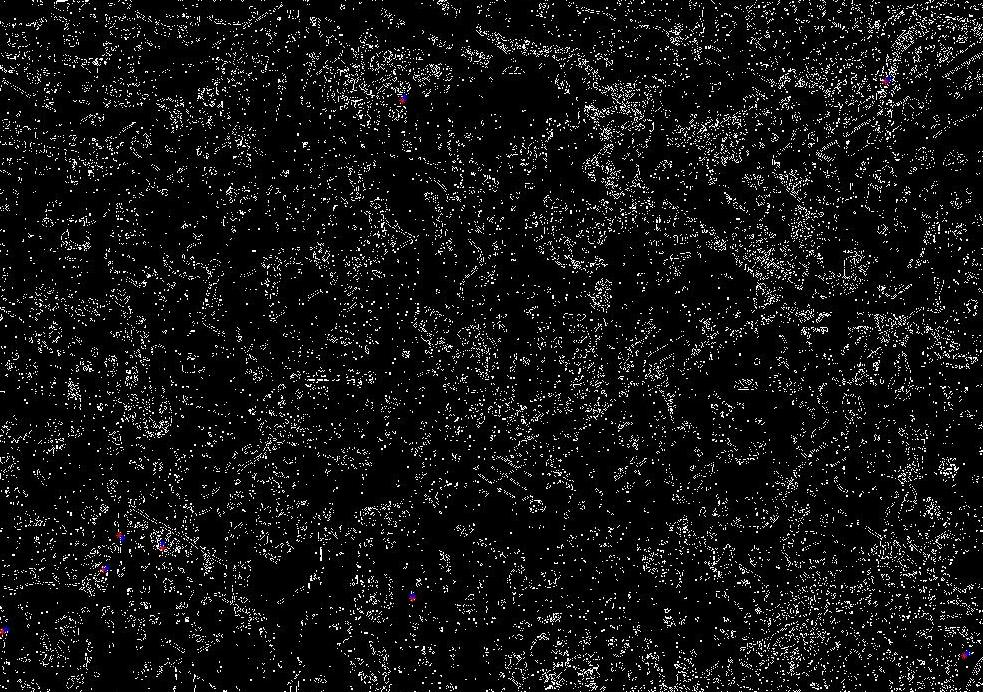
\includegraphics[width=0.9\textwidth]{img/glasses_2_wholeWembley.jpg}
  \caption{8 Mutmassliche Augapfel Paare}
  \label{fig:Bild1}
\end{figure}
%\begin{SCfigure}
%  \centering
%  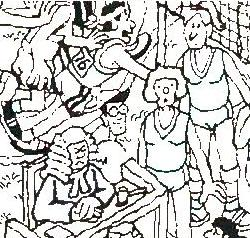
\includegraphics[height=.4\linewidth]{img/glasses_blackExtract.jpg}
%  \caption{}
%\end{SCfigure}
%\begin{SCfigure}
%  \centering
%  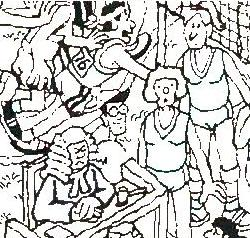
\includegraphics[height=.4\linewidth]{img/glasses_blackExtract.jpg}
%  \caption{Um die Ränder der Brille zu schliessen wurde ein binäres Closing angewandt.}
%\end{SCfigure}
\newpage
\subsection*{T-Shirt}
Das Walters T-Shirt aus weissen und roten Streifen besteht, wurde versucht einen zusammenhängenden Bereich aus roten und weissen Teilen zu finden.

\descFig{img/tshirt_whiteExtract.jpg}{Extraktion der weissen Farbe}{Zuerst wurden die weissen Pixel extrahiert. Das heisst die Pixel, bei welchen alle 3 RGB Kanäle Werte grösser als 0.8 besitzen.}

\descFig{img/tshirt_redExtract.jpg}{Extraktion der roten Farbe}{Anschliessend wurden die roten Pixel extrahiert. Das heisst die Pixel, bei welchen der Rotkanal doppelt so gross ist, wie das Maximum des Grün- und Blaukanals.}

\descFig{img/tshirt_whiteRedExtract.jpg}{Extraktion der roten und weissen Farbe}{Im nächsten Schritt wurden die roten und weissen Pixel zusammengefügt.}

\descFig{img/tshirt_whiteRedDilated.jpg}{Dilatation}{Anschliessend wurde das Bild dilatiert um die Lücken zwischen den Streifen zu schliessen.}

\descFig{img/tshirt_connected.jpg}{Verbundene weiss/rote Fläche}{Im letzten Schritt wurde mittels Region-Growing Flächen gesucht, die rote und weisse Pixel enthalten. Zu diesem Zweck wurde über das Bild geloopt. Sobald ein rotes oder weisses Pixel gefunden wurde, wurde von diesem aus das Region-Growing gestartet. Dabei wurden die roten und weissen Pixel zur Fläche hinzugefügt. Für die hinzugefügten Pixel wurden wieder deren Nachbarn überprüft. Sobald eine Fläche vollständig gefunden wurde, wurde überprüft ob die Fläche sowohl rote als auch weisse Pixel enthält. War dies der Fall wurde die Fläche zum Resultat-Bild hinzugefügt, ansonsten wurde die Fläche verworfen.}

Auf das ganze Bild angewandt ergibt sich folgendes Bild.
\begin{figure}[htbp] 
\centering
  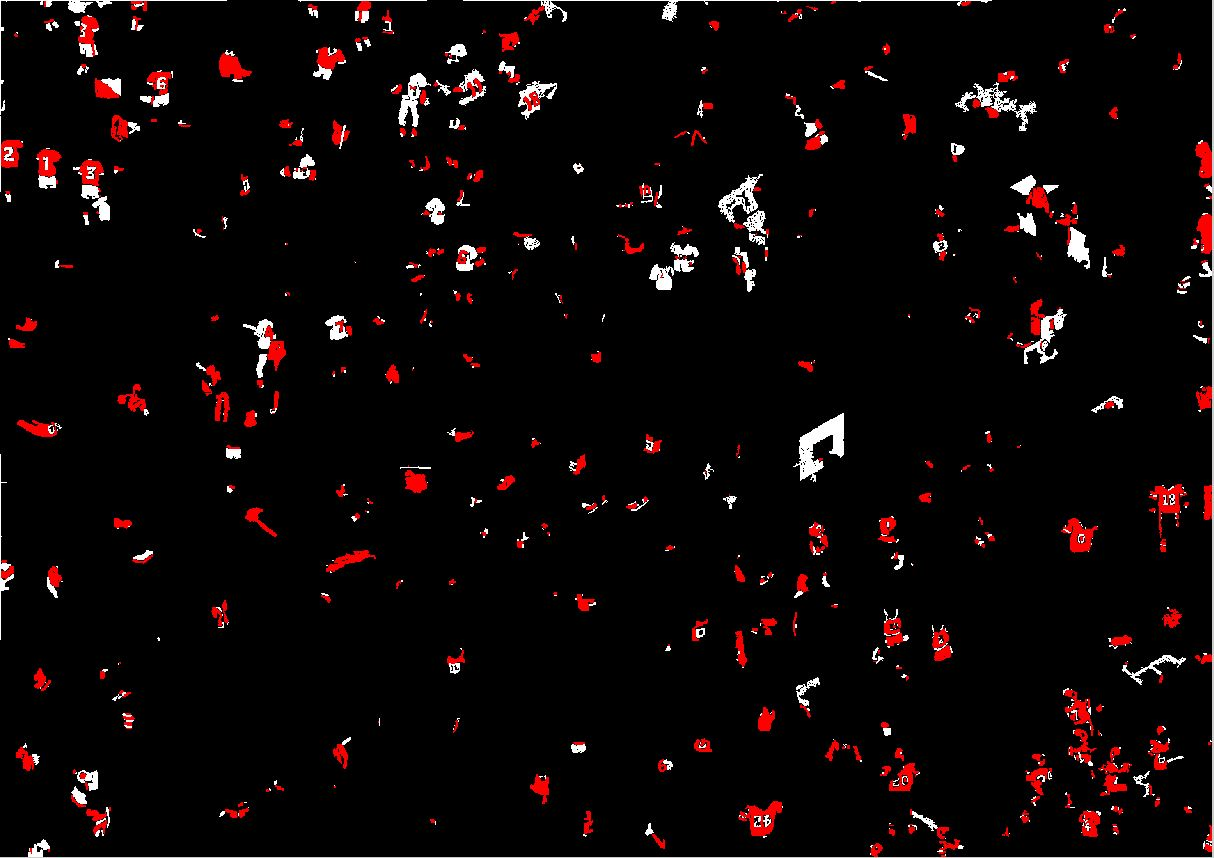
\includegraphics[width=0.9\textwidth]{img/tshirt_connectedFull.jpg}
  \caption{Verbundene weiss/rote Fläche}
  \label{fig:Bild1}
\end{figure}

\newpage
\section*{Ergebnisse, Resultate}

\end{document}
